% Questions on PDF page 134
\documentclass[11pt]{article}

\usepackage[utf8]{inputenc}
\usepackage[a4paper, margin=.8in]{geometry}
\usepackage{booktabs}
\usepackage{enumerate}
\usepackage{physics}
\usepackage{amsmath}
\usepackage{amsfonts}
\usepackage{graphicx}
\usepackage{siunitx}
\usepackage{textcomp}
\usepackage{makecell}
\usepackage{hyperref}
\usepackage{multicol}
\usepackage{float}
\usepackage{multirow, tabularx}

\bibliographystyle{ieeetr}
\graphicspath{{./figures}}

%\title{Big Data (AES 630) Homework 3}
%\author{Mitchell Dodson}
%\date{February 22, 2024}

\newcommand*{\problem}[2]{
    \begin{table}[ht]
    \centering
        \begin{tabular}{ | p{.1\linewidth} p{.9\linewidth} | }
            \hline
            \vspace{.3em}\textbf{\large#1:} & \vspace{.3em}\small{#2}\hspace{.2em}\vspace{.5em} \\ \hline
        \end{tabular}
    \end{table}
}

\begin{document}

\noindent
{\Large\textbf{Deep Learning Approaches for Efficiently Emulating Noah Land Surface Model Soil Hydrology}}

\vspace{.8em}

\noindent
\large{Master's Thesis Proposal}

\noindent
\large{Mitchell Dodson}

\vspace{-.8em}

\section{Introduction and Hypothesis}

Accurate characterization of land surface states including profiles of soil moisture and temperature are fundamental to numerical weather prediction, crop health and hydrologic monitoring, and for situational awareness during drought and flood events. To that end, the Noah Land Surface Model (Noah-LSM) has become a fixture in the numerical modeling and operational forecasting communities, serving as the land component of the Weather Research and Forecasting (WRF) community model, NOAA's Global Forecast System (GFS) and Climate Forecast System (CFS) models, and as a near real-time product utilized by the National Weather Service and US Drought Monitor \cite{xia_continental-scale_2012}\cite{sorooshian_ncep_2005}\cite{mccartney_application_2023}.

High spatial resolution and the ability to generate land surface states from ensembles of atmospheric forcings are high priorities for forecasting and reanalysis frameworks including the next-generation North American Land Data Assimilation System (NLDAS) \cite{ek_next_2017}\cite{mocko_preparing_2023}. Like many dynamical models, evaluating Noah-LSM over large spatial or temporal domains is computationally costly since it relies on recurrent numerical integration techniques which can be difficult to parallelize. Deep learning techniques provide the means to approximate a highly nonlinear and heavily parameterized system like Noah-LSM by inferring the relationship between input and output values in a set of training samples, and encoding their dynamics as a sequence of composed affine matrix operations followed by nonlinearities, which are computationally efficient on modern GPU hardware \cite{lecun_deep_2015}\cite{russell_artificial_2010}. As such, this proposal hypothesizes that a deep learning model trained on atmospheric forcings and model outputs from NLDAS-2 \cite{xia_continental-scale_2012} can simulate the soil hydrodynamics of the Noah model with low computational cost and fidelity sufficient enough to provide useful estimates.

\section{Background}

\begin{multicols}{2}

    \subsection{The History of Noah-LSM}

    The theoretical framework underpinning Noah-LSM was initially formulated in the 1980s as part of the OSU model, which characterizes boundary layer moisture and energy fluxes as a 2-layer soil model subject to atmospheric forcings. The model expresses the infiltration and movement of water between the soil layers with the diffusive form of the Richards equation \cite{mahrt_two-layer_1984}, direct evaporation using an analytic approximation of the Penman-Montieth relation in terms of atmospheric stability \cite{mahrt_influence_1984}, and basic plant transpiration in terms of vegetation density and soil water content \cite{pan_interaction_1987}. These features form an interdependent system of differential equations that are numerically integrated using a combination of the Crank-Nicholson method and finite-differencing \cite{chen_impact_1997}, which introduces the need for short time steps of 15 or 30 minutes in order for the system to remain numerically stable \cite{cartwright_dynamics_1992}\cite{mahrt_two-layer_1984}.

    \begin{figure}[H]
        \centering

        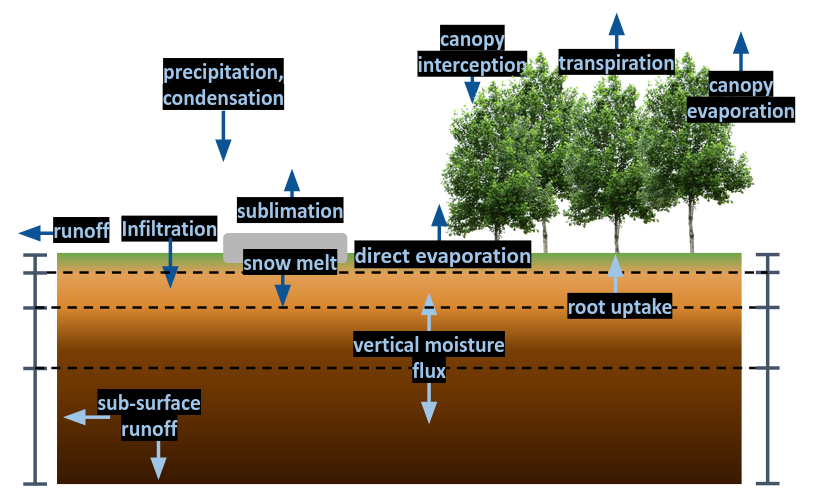
\includegraphics[width=.98\linewidth]{figs/noah-hydrology.png}

        \caption{Schematic diagram of the feedbacks contributing to the evolution of volumetric soil moisture in Noah-LSM}
        \label{feedback_schematic}
    \end{figure}

\end{multicols}

\begin{figure}[h!]
    \centering

    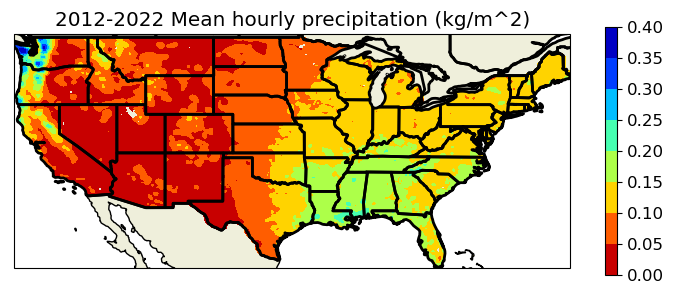
\includegraphics[width=.48\linewidth]{figs/mean_precip.png}
    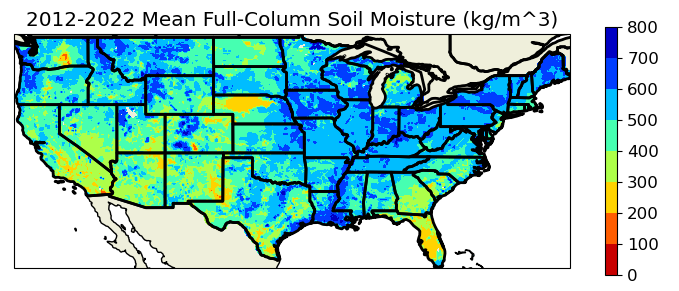
\includegraphics[width=.48\linewidth]{figs/mean_soilm_full.png}

    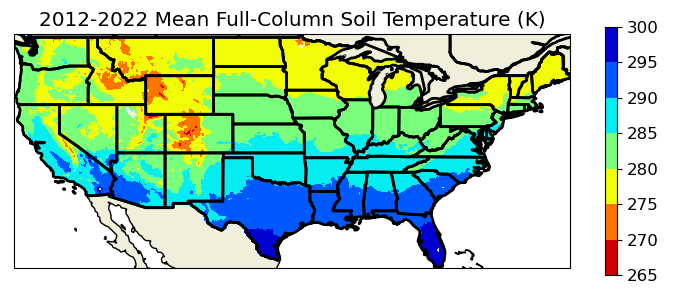
\includegraphics[width=.48\linewidth]{figs/mean_tsoil_full.png}
    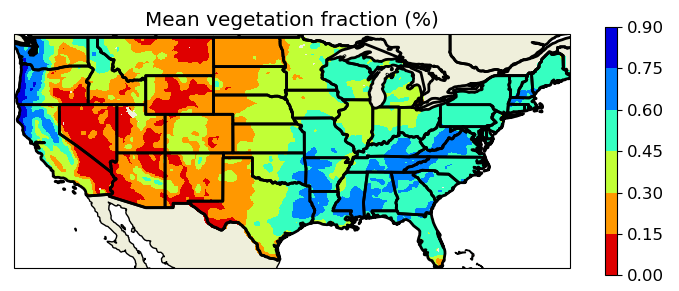
\includegraphics[width=.48\linewidth]{figs/mean_vegfrac.png}

    \caption{NLDAS-2 mean values over study period. Clockwise: hourly precipitation (either phase), full-column (2m) soil moisture, vegetation fraction, and full-column soil temperature.}
    \label{mean_samples}
\end{figure}

\begin{multicols}{2}

    The OSU model was later significantly improved, renamed to the first generation of Noah-LSM, and coupled with the NCEP Eta forecast model. Noah-LSM expanded the domain to four soil layers of increasing thicknesses 10cm, 30cm, 60cm, and 100cm, improved runoff dynamics by implementing Philip's equation for infiltration capacity \cite{schaake_simple_1996}, and represented influence of soil texture on moisture transport by introducing bounds on bare-soil potential evaporation that are determined by the soil composition \cite{betts_assessment_1997}\cite{mahfouf_comparative_1991}. The model also features a significantly enhanced representation of vegetation including a more thorough treatment of canopy resistance via a ``Jarvis-type'' model of leaf stomatal control \cite{jarvis_interpretation_1976}\cite{jacquemin_sensitivity_1990}, which accounts for the dependence of transpiration on insolation, air temperature and dewpoint, soil moisture capacity, and vegetation density. The vegetation effects are scaled by a monthly climatology of normalized difference vegetation index (NDVI) values observed by the NOAA-AVHRR satellite radiometer, which serve as a proxy for green vegetation fraction (GVF) \cite{gutman_derivation_1998}\cite{chen_modeling_1996}, and the depth of root water uptake associated with plant transpiration is determined by a pixel's vegetation class as specified by the Simple Biosphere Model \cite{dorman_global_1989}. Finally, the model's utility was greatly expanded with the addition of a frozen soil and snow pack parameterization incorporating the thermal and hydraulic properties of fractionally-frozen soil layers, the effects of state changes \cite{chen_modeling_1996}\cite{koren_parameterization_1999}, radiative feedbacks from partial snowpack coverage, and a snow density scheme \cite{ek_implementation_2003}.

    \subsection{NLDAS and Noah-LSM}

    Soon after the turn of the millennium, the first generation of NLDAS was under development as part of a multi-institution collaborative effort sponsored by the Global Energy and Water Cycle Experiment (GEWEX) Continental-scale International Projects (GCIP) team. The goal of the project was to incorporate long-term observations of land surface temperature, snow pack depth, and meteorological forcings from multiple sources (in-situ, satellite, radar) into a common framework used to independently evaluate land surface states and energy fluxes with four land surface models including Noah-LSM \cite{mitchell_multi-institution_2004}. On a domain including the full conterminous United States (CONUS) at $0.125^\circ$ resolution, the models were allowed to spin up over the course of a year, and soil states were recurrently used to initialize subsequent time steps rather than being ``nudged'' to correct for drift. Land cover and soil texture classification over the domain was derived by coarsening the University of Maryland and STATSGO datasets, respectively, from their native 1km resolutions \cite{hansen_global_2000}, surface geometry and elevation is provided by the GTOPO30 dataset \cite{earth_resources_observation_and_science_centeru_s_geological_surveyu_s_department_of_the_interior_usgs_1997}, and the parameter values for soil hydraulic properties were adapted from observations taken at the University of Virginia \cite{cosby_statistical_1984}.

\end{multicols}

\begin{table}[h!]
    \centering
    \begin{tabular}{ l l l l l}
        Forcing & Unit & Source & $\Delta$t & $\Delta$x \\
        \hline
        Temperature & K & NCEP fta/EDAS & 3h & 40km \\
        Specific Humidity & kg kg$^{-1}$ & NCEP Eta/EDAS & 3h & 40km \\
        Wind Velocity & m s$^{-1}$ & NCEP Eta/EDAS & 3h & 40km \\
        Downward Longwave Flux & W m$^{-2}$ & NCEP Eta/EDAS & 3h & 40km \\
        Downward Shortwave Flux & W m$^{-2}$ & UMD GOES-based insolation & 1h & 55km \\
        %Potential Evaporation & kg m$^{-2}$ & Calculated from Penman-Montieth relation \\
        \multirow{2}{*}{Precipitation} & \multirow{2}{*}{kg m$^{-2}$} & Gauge observations & 24h & 14km \\
        & & WSR-88D radar retrievals & 1h & 4km \\
    \end{tabular}
    \caption{Atmospheric forcings provided by NLDAS at a 1-hourly resolution on the $0.125^\circ$ CONUS grid. Data are resampled using spatial bilinear interpolation, then temporal disaggregation \cite{mitchell_multi-institution_2004}. NLDAS forcing files also include values for CAPE, the ratio of convective precipitation, and potential evaporation (calculated as in \cite{mahrt_influence_1984}), but these three values won't be used as inputs to the models.}
    \label{forcing}

\end{table}

\vspace{-1.2em}

\begin{multicols}{2}

    Attention remained on Noah-LSM in the following years as it continued to support NLDAS and other data assimilation and forecasting systems, which led to a series of improvements introduced alongside the next phase of the NLDAS project. A seasonal effect was added to vegetation by scaling the leaf area index (LAI) by GVF within bounds determined by the plant type, and transpiration was scaled by a root uptake efficiency factor determined by the proximity of soil temperature to an optimum growth temperature (298 K).

    Several parameters were adjusted including the influence of vapor pressure deficit on transpiration rate, the minimum stomatal resistance for several plant species, and hydraulic parameters for some soil textures. The aerodynamic conductance coefficient -- an important factor in the strength of moisture and energy fluxes from the surface -- was increased during daylight hours, and a basic anisotropy model was introduced by modifying the albedo of some surfaces in terms of the solar zenith angle \cite{wei_improvement_2011}. Snowpack physics were also modified to improve surface exchange coefficients, and to gradually diminish the snow albedo over the time since the last snowfall \cite{livneh_noah_2010}\cite{liang_simple_1994}. These changes introduce new feedbacks and involve sensitive parameters like LAI which have a strong influence on the model's dynamics \cite{rosero_quantifying_2010}.

    The retrospective NLDAS-2 data record generated after applying these modifications extends back to 1979, and continues to be updated in a near real-time capacity \cite{xia_continental-scale_2012}. Its forcings listed in Table \ref{forcing} serve as the inputs to the neural networks, which are trained to predict the associated Noah land surface model states minimally including soil moisture and snow water equivalent.


    \subsection{Noah as a Dynamical Model}

    At its core, Noah-LSM is a collection of differential equations that express the time rate of change of land surface states $\frac{\partial \vec{s}}{\partial t}$ in terms of the current state $\vec{s}$, forcing $\vec{\psi}$, and parameters $\vec{\phi}$. Here, $\vec{s}$ consists of the model's dynamic state variables (snow pack depth, soil moisture and temperature, canopy storage), $\vec{\psi}$ encodes forcings from Table \ref{forcing}, and $\vec{\phi}$ includes static coefficients of the governing equations (ex. vegetation type/fraction, soil texture, elevation).

    \begin{figure}[H]
        \centering

        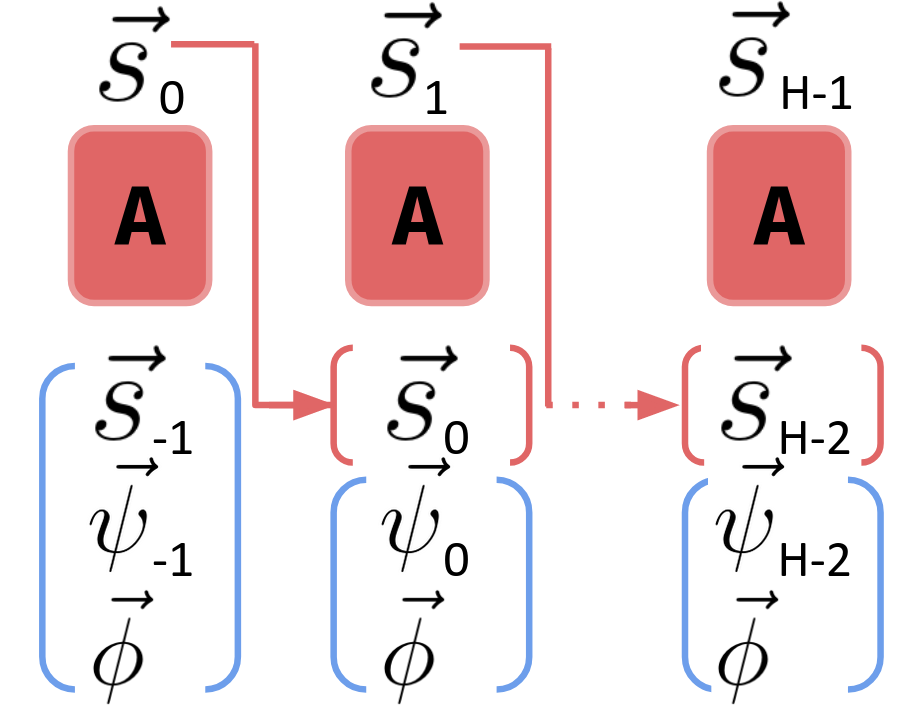
\includegraphics[width=.66\linewidth]{figs/abstract_scann.png}

        \caption{Diagram of a self-cycling discrete-time dynamical system with no hidden state. At each time, nonlinear operator \textbf{A} maps an initial state $\vec{s}_k$, exogenous forcing $\vec{\psi}_k$, and time-invariant parameters $\vec{\phi}$ to a new state $\vec{s}_{k+1}$, used to initialize the subsequent time step.}
        \label{scann}
    \end{figure}

    \vspace{-1.2em}

    To generate a time series, Noah-LSM numerically integrates the system of equations using Euler and Crank-Nicholson techniques, which explicitly evaluate the differential equations at several time intervals in order to estimate the residual change in state while conserving the appropriate quantities. It is crucial that the time step remains small (15min for NLDAS-Noah) to mitigate truncation error from the assumption of local linearity \cite{mitchell_multi-institution_2004}\cite{cartwright_dynamics_1992}.

\end{multicols}

\begin{figure}[h!]
    \centering

    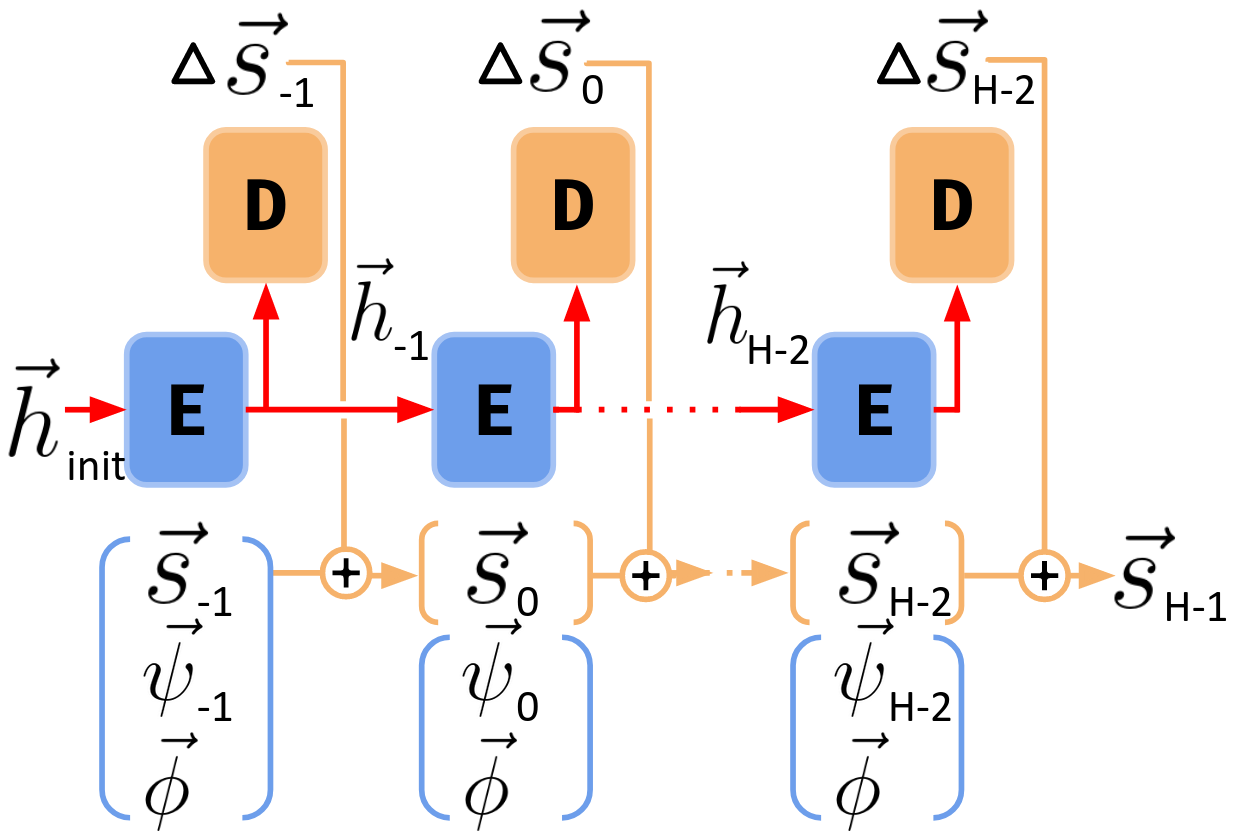
\includegraphics[width=.38\linewidth]{figs/abstract_scrnn.png}
    \hspace{3em}
    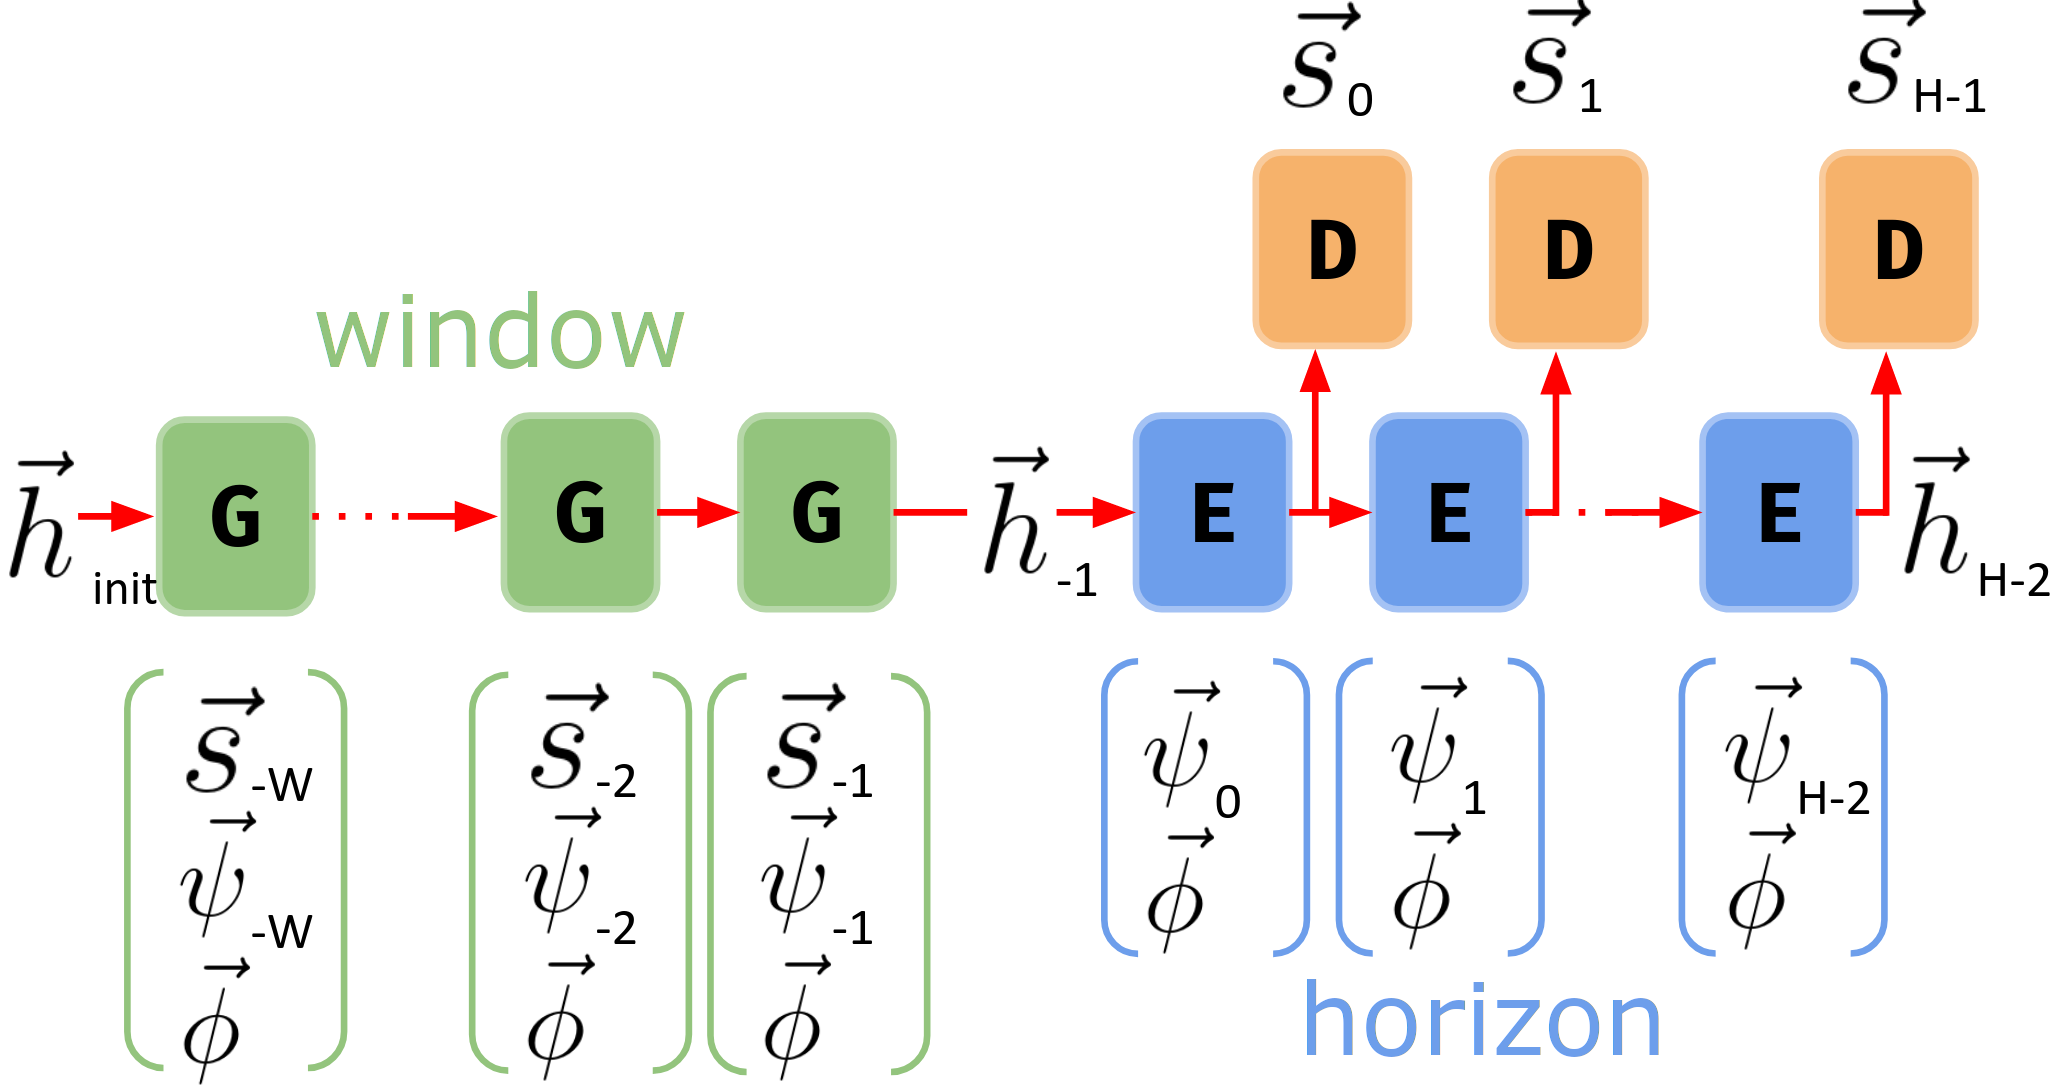
\includegraphics[width=.50\linewidth]{figs/abstract_rnn.png}

    \caption{Information flow diagrams for a basic self-cycling RNN (left) and a sequence-to-sequence RNN (right). Both models have an encoder \textbf{E} that transforms current inputs and the previous hidden state into a new hidden state, then use a decoder \textbf{D} to generate outputs for H discrete time steps in the ``forecast horizon.'' The sequence-to-sequence RNN features a separate encoder \textbf{G} that uses a series of prior values to initialize the hidden state used in prediction steps.}
    \label{rnns}
\end{figure}

\begin{multicols}{2}

    Figure \ref{scann} provides a general schematic that applies to Noah's evaluation process. Although no information is propagated between time steps by the model (except the output state), hysteretic effects emerge from the dynamics of \textbf{A} when it is numerically integrated. For example, the characteristic curves of unsaturated soil moisture diffusion depend on the timing of periods of wetting and dry-down since drainage and infiltration rates have a nonlinear relationship to the moisture content in the Richards equation \cite{jaynes_comparison_1984}.

    \subsection{Deep Learning Approach}

    As discussed in the previous section, the goal of numerical integration is to approximate the continuous evolution of a dynamical system by applying an explicit and highly nonlinear equation over small discrete time steps. Neural networks have effectively the opposite approach, in that they use many sample time series (generated by the model) to learn the governing equations implicit to the samples' dynamics.

    Deep neural networks are a reasonable strategy for creating a reduced-order simulation of Noah-LSM's dynamics because they are universal function approximators, which means that given a sufficient number of learnable weights, a feedforward network with at least one hidden layer (two composed linear matrix operations each followed by an element-wise nonlinear function) can learn an arbitrary decision boundary or multivariate function \cite{hornik_multilayer_1989}. This high level of expressivity enables the network to learn complex relationships and generalizations among high-dimensional parameters given repeated exposure during training.

    Although a simple feed-forward neural network (FNN) is theoretically capable of simulating Noah-LSM in the manner of Figure \ref{scann}, inductive biases are commonly introduced in model architectures in order to promote efficiency, explainability, stability, and parsimony. For example, most neural networks used for sequence modeling like the recurrent neural networks (RNNs) in Figure \ref{rnns} maintain a ``hidden'' latent parameter $\vec{h}$ with an arbitrary number of dimensions. This vector is modified and passed along by each subsequent iteration, giving the network the ability to make generalizations and propagate information between time steps. Although $\vec{h}$ is typically difficult to interpret directly, the gradient descent process incentivizes the network to preserve and consolidate information that is needed to accurately generate the full sequence of predictions. Each of the following network architectures ultimately aim to improve the information quality of the latent vector by implementing algebraic structure, introducing statistical uncertainty, and encouraging sparsity.

    \begin{equation}\label{eq_rnn}
        \begin{split}
            \vec{h}_k &= \mathbf{E}(\vec{h}_{k-1}, \vec{s}_k, \vec{\psi}_k, \vec{\phi}) \\
            \vec{s}_{k+1} &= \vec{s}_{k} + \mathbf{D}(h_k)
        \end{split}
    \end{equation}

    The RNNs discussed here will follow the structure described by Equation \ref{eq_rnn}, so that the decoder output is a prediction of the residual change in the state rather than the absolute magnitude of the next state. Previous experiments with this project suggested that this improves model stability, and enables the model loss to balance local error in the residual with global error from the new state (which is vulnerable to accumulation) \cite{he_deep_2015}. The most basic RNNs implement their encoder and decoder modules each as a FNN such that the latent state $\vec{h}_k$ is output directly by the final layer of the encoder, and then decoded to the output.

    The basic RNN architecture is vulnerable to the so-called vanishing or exploding gradient problem, which arises from the fact that $\vec{h}_k$ is the product of a learned matrix operation. Since the encoder and decoder weights are shared between sequence steps, the backpropagation through time algorithm may update a parameter many times per sample during training, which can cause weights to diverge and cease learning \cite{mozer_focused_1995}. Furthermore, since the hidden state undergoes a nonlinear transformation at each step, it is difficult for the network to sustain information over a long context of past observations.

    \begin{figure}[H]
        \centering

        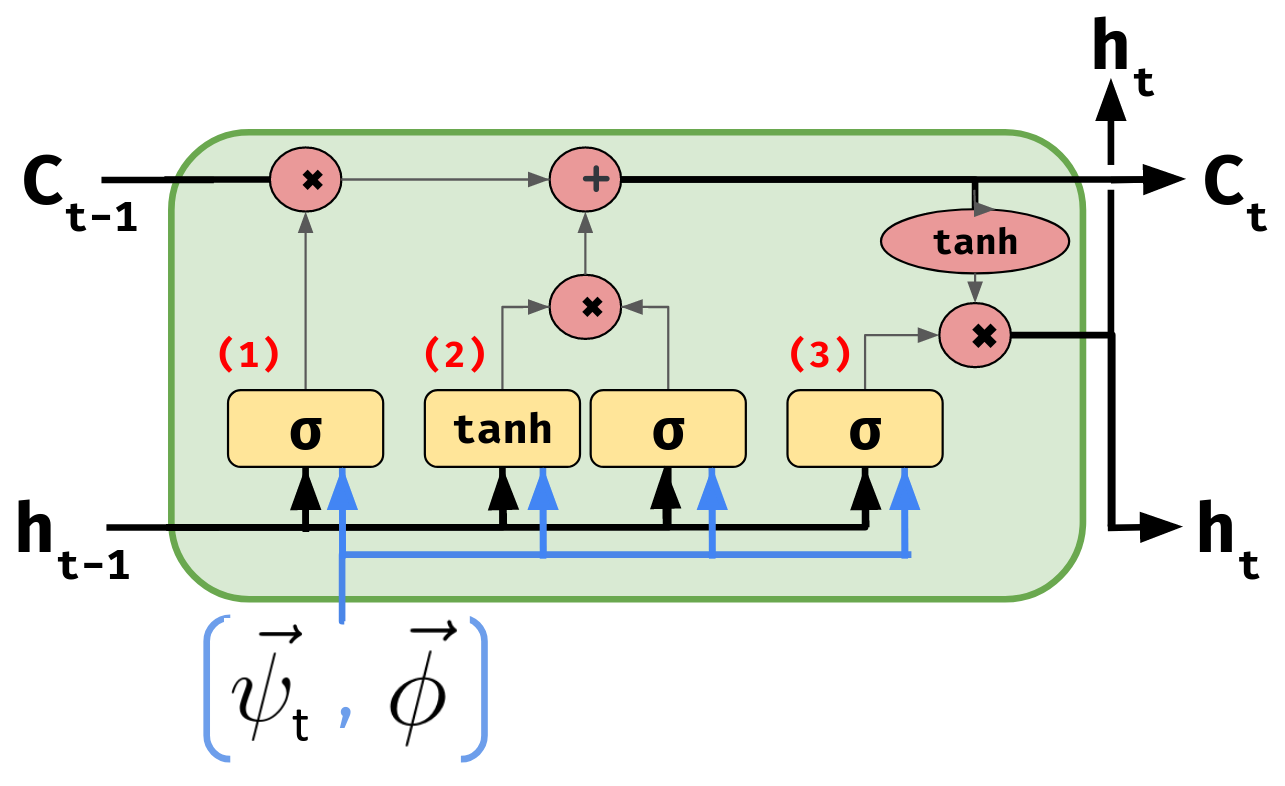
\includegraphics[width=.8\linewidth]{figs/lstm.png}

        \caption{Long Short-Term Memory module. The previous latent vector $\vec{h}_{t-1}$ and inputs $\vec{\psi}_t$, $\vec{\phi}$ are used to select coefficients for linearly scaling the context vector $C_{t-1}$, then the inputs and updated $C_t$ are used to generate the new latent vector $h_t$.}
        \label{lstm}
    \end{figure}

    The Long Short-Term Memory (LSTM) architecture addresses these shortcomings by maintaining a separate hidden state $\vec{C}_t$ called the context vector. Rather than being generated by a matrix operation, the context vector is only modified by the output of a series of three ``gates.'' These gates (numbered in Figure \ref{lstm})  include (1) the ``forget gate'', which uses a FNN to select a vector of values in the range (0,1). The vector is multiplied element-wise by $\vec{C}_{t-1}$ in order to selectively emphasize or diminish its activation. The ``update gate'' (2) transforms the inputs into a new coefficient vector in the range (-1,1), which is added to the context vector in order to retain information from the current time step. Finally, the ``output gate'' (3) generates a vector of multiplicative coefficients in the range (0,1) used to scale the new context vector $\vec{C}_t$ to the output latent state $\vec{h}_t$ \cite{hochreiter_long_1997}. The context vector remains stable compared to a hidden vector that is recurrently operated on by the same weight matrix, which facilitates the network to learn over a longer sequence interval.

    \begin{figure}[H]
        \centering

        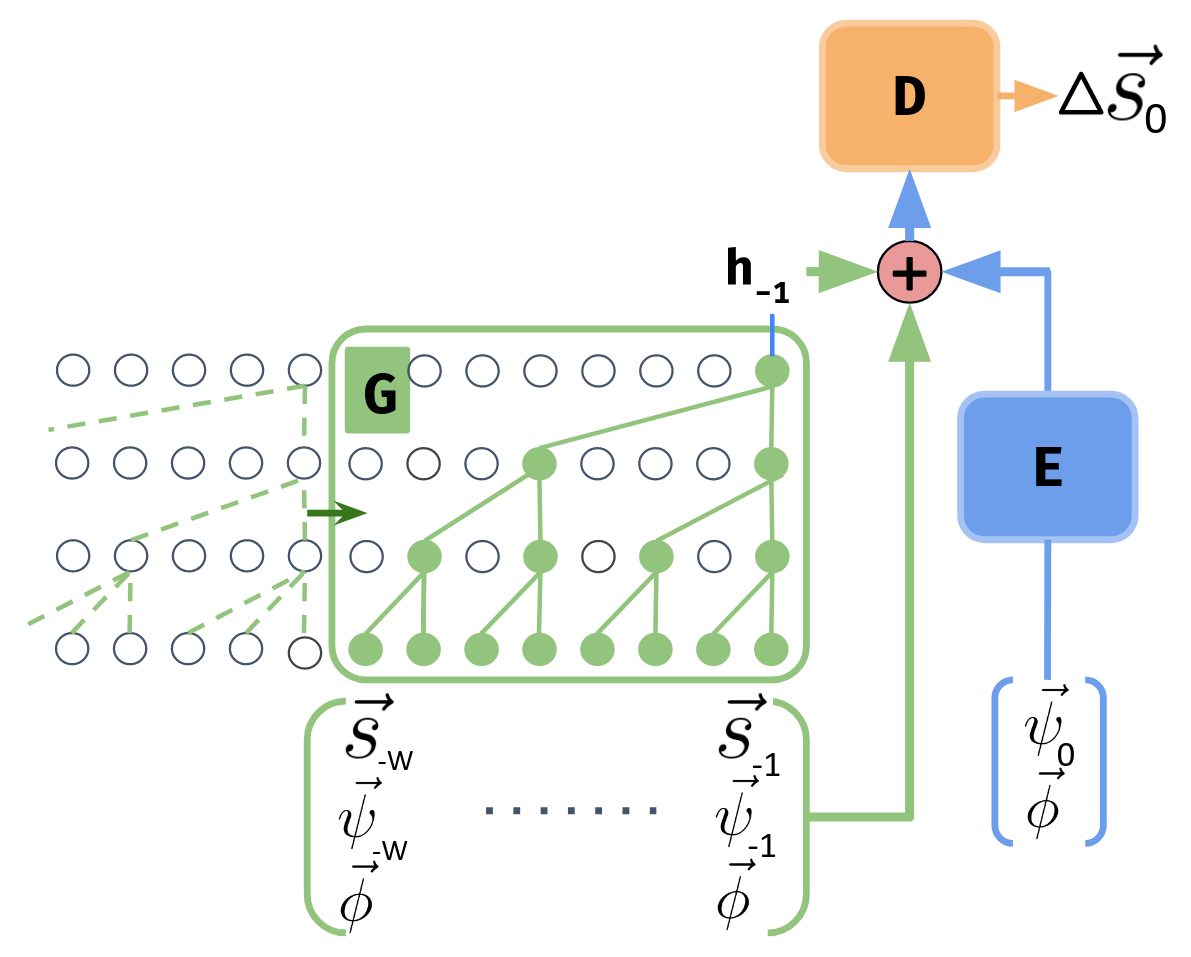
\includegraphics[width=.95\linewidth]{figs/deeptcn.png}

        \caption{Deep Temporal Convolutional Network module, featuring three layers of dilated 1D convolutions for encoding previous time steps, a FNN-based residual encoder \textbf{E} for incorporating information from forcing variables, and a FNN decoder \textbf{D} that generates the residual state change.}
        \label{deeptcn}
    \end{figure}

    Rather than maintaining a persistent latent vector between sequence steps, an alternative approach is to expose each timestep to the full sequence of past states. This is difficult to implement using traditional FNN modules since model complexity would scale quadratically with sequence length. The Deep Temporal Convolutional Network (DeepTCN) addresses this with dilated convolutions, which expand the receptive field of the encoder exponentially with depth. Next, skip connection from the latest input step is added to the hidden vector, and the exogenous forcings associated with the prediction steps are encoded and added to the latent vector. Finally, the hidden vector is decoded to a prediction \cite{chen_probabilistic_2020}. As the dilated convolutional filters slide across the input sequence, each element in the latent sequence they generate is only exposed to past information, and has an implicit causal ordering from the kernel's structure. These properties grant the model a sense of temporality that may help it infer high-level patterns \cite{oord_wavenet_2016}. In this problem context, the DeepTCN could serve as an encoder that recurrently cycles its previous state predictions, or as a decoder that generates predictions from a latent sequence. Previous testing suggested that this architecture is the most promising for stably generating short-term dynamics at an hourly resolution.

    \begin{figure}[H]
        \centering

        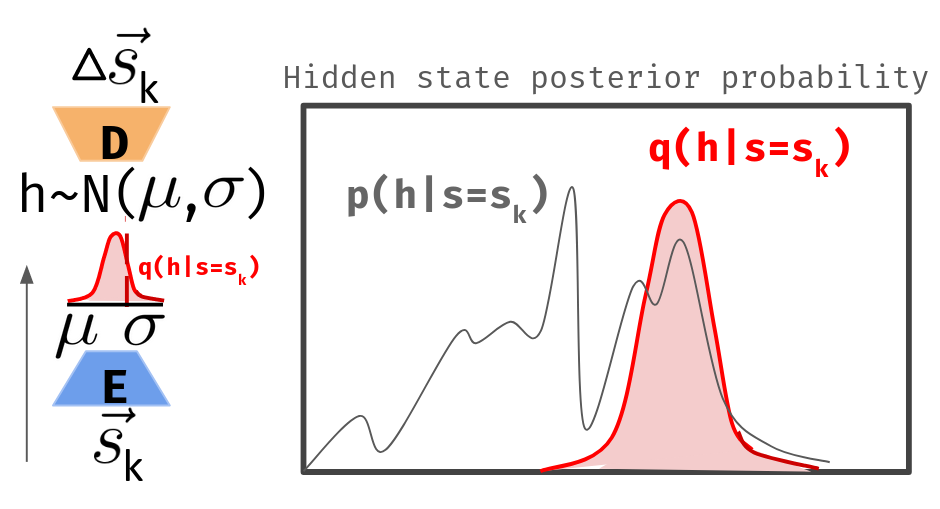
\includegraphics[width=.95\linewidth]{figs/ved.png}

        \caption{(left) Schematic overview of the variational encoder-decoder procedure. The encoder \textbf{E} produces vectors of coefficients parameterizing analytic distributions (ie mean and variance describing a standard normal distribution N). An independent random variable is used to sample a latent vector $\vec{h}$ from the distribution in accordance with its parameters. Finally, the chosen $\vec{h}$ is provided to the decoder \textbf{D}, which converts it back to the original state space to generate the residual. (right) The encoder's approximate posterior distribution $q(\vec{h}|s=s_k)$ over the latent vector space is selected by the encoder based on the input state $\vec{s}_k$. The encoder aims to use the previous-state information $\vec{s}_k$ to restrict the domain of valid latent activations to a simple distribution, which is a subspace of the intractable true posterior distribution $p(\vec{h}|\vec{s}=\vec{s}_k)$.}
        \label{ved}
    \end{figure}

    The final model type considered here are variational encoder-decoders, which enable models to explicitly characterize their uncertainty by generating parameters for analytic surrogate distributions $q(\vec{h}|\vec{s}=\vec{s}_k)$ over the latent space. The parameters are optimized to approximate the true posterior distribution of valid latent space activations given the input state $s_k$. During training, the model fits the surrogate distributions by seeking to minimize the Kullback-Leibler divergence between the two distributions, thereby minimizing their relative entropy. Backpropagation through the distribution is made possible by the so-called ``reparameterization trick,'' which stochastically samples a latent vector according to the predicted distribution using an independent random variable. This simulates the posterior in terms of a Monte-Carlo estimator given many training samples \cite{kingma_auto-encoding_2014}\cite{ganguly_amortized_2023}.

    There are several benefits to the variational approach. First, since local uncertainty in the latent space is explicitly encoded during training, variational models tend to be more spatially coherent, and tend to find more parsimonious representations of their dynamics \cite{lopez_gd-vaes_2022}\cite{kutz_parsimony_2022}. This often means that a family of valid outputs can be generated by smoothly interpolating between two latent vectors. The approximate posterior distribution produced by the encoder can also be easily used to generate an ensemble of outputs according to the model's intrinsic uncertainty, which can enhance explainability. Finally, hidden states parameterized by variational distributions can be applied to any of the previous architectures as a means of improving latent space dynamics. For instance, an LSTM encoder could generate parameters to a distribution for each of its sequence outputs, which are individually sampled during inference, or a decoder could output a variational distribution that makes explicit the uncertainty in its residual.

    The Transformer architecture has dominated many sequence modeling tasks in recent literature thanks to the key innovation of multi-head self-attention (MSA), which enables the architecture to learn complicated relationships between individual members of the input sequence regardless of their relative position. Additionally, transformers are efficient to train in parallel, unlike RNN-style architectures which rely on a chain of sequential operations, which makes them straightforward to train on a massive scale \cite{vaswani_attention_2017}. The results for natural language processing (NLP) \cite{devlin_bert_2019} and image classification \cite{dosovitskiy_image_2021} tasks are impressive, however there are several key drawbacks that make them less appealing for a time series generation task like this one. First, the memory cost of a transformer scales quadratically with sequence length since MSA learns parameters relating every possible combination of input steps. This is compounded with the fact that the full input sequence needs to be re-initialized with every step during inference. These properties are a direct trade-off with the Transformer's ability to train separate sequence steps in parallel. Furthermore, unlike RNNs and CNNs, Transformers don't have an inherent notion of order. In problems like NLP where sequence position conveys some information, a simple form of locality is introduced by adding a positional embedding vector directly to the inputs. Nonetheless, prior literature shows that transformers equipped with positional embedding still perform no better on basic time series forecasting tasks than a simple 2-layer FNN \cite{zeng_are_2022}.

\end{multicols}

\section{Procedure}

\begin{multicols}{2}

\subsection{Dataset Curation}

    The data used for this project is retrieved from the NLDAS-2 climatology available on NASA Goddard's GES DISC archive, where it is stored as a collection of GRIB-1 files for each hourly time step on a 225x464 spatial grid. So far, the 10 years between 2012 and 2022 have been acquired for model training and testing, but this can be expanded to a larger interval for further testing. Each time step has separate files for NLDAS-2 forcing and the subsequent Noah-LSM model run, both of which contain several superfluous data values.

    It isn't feasible to train models directly from data read from the GRIB files since generating a set of multi-day single-pixel sequences by sparsely sampling files from a 10-year record would require hundreds of files to be opened and preprocessed in quick succession during training, which is computationally prohibitive. An intermediate format for storing and retrieving data is needed, which should be able to quickly index data across time.

    The HDF5 format provides the ability to store a tree of multidimensional arrays in a compressed format, and to memory-map user-specified chunks for efficient cached retrieval from storage. At this stage, it's helpful to store the dynamic data (forcings, model outputs), static data (parameters and masks), and spatial/temporal coordinates together with unique labels assigned to each feature. This structure makes it easy to retrieve perform operations on arbitrary subsets of data given coordinate bounds and an ordered set of labels. The requisite metadata for interacting with N-dimensional arrays this way can be JSON-serialized and reloaded from the HDF5s using a Python interface I call the FeatureGrid.

    In practice, each individual HDF5 represents a 3-month interval of data from a region covering 1/6 of the CONUS domain. The files contain a (N, P, Q, F$_D$) array of dynamic features F$_D$ on a PxQ pixel subset of the domain, measured at N consecutive time steps, a (P, Q, F$_S$) array of F$_S$ static features on the same grid, and a (N, F$_T$) array of temporal but spatially-invariant features F$_T$ (ie timestamp, solar zenith angle). The arrays will be organized in memory so that each chunk contains 8 features observed at 256 hours ($\sim$11 days) over a 32x32 pixel region. The size of each chunk is about 10.5MB, and the full size of each regional HDF5 file is about 3GB. This chunking strategy is useful because it promotes quick extraction of long time series needed for training without loading the full file into memory, and without compromising access to the spatial structure needed for analysis and visualization.

    Before the data can be used to train and evaluate the models, it still needs to be sampled, preprocessed, and reshaped to the format expected by the model. This procedure is implemented using Python generators, which are able to produce the curated data on-demand by memory-mapping many HDF5 files in parallel and generating samples according to user settings. Since the generators are initialized at training time, model parameters like input/output variables, normalization bounds, and sequence length can be specified last-minute by the training configuration. During model development, it is also advantageous to be able to constrain the data population that training samples are drawn from. For example, models may be trained on a simplified problem by only sampling sandy-soil pixels in a spatially bounded region during the summer, or a model could be evaluated with respect to each vegetation type independently. The generators will open the HDF5 data as FeatureGrid objects, which provide the ability to restrict the data to a subset based on conditional constraints like these, then the generator will extract a shuffled batch of samples from the remaining domain.

    After being normalized (typically by linearly scaling the data to a standard gaussian), the batch is yielded by the sample in the format expected by the models. The model input is a 3-tuple of arrays consisting of a (B, L$_W$, F$_W$) array of B samples of F$_W$ dynamic features in the spin-up `window' sequence of length L$_W$ ($\vec{\psi}_k$, $\vec{s}_k$ for $k \in [-L_W,0)$), a (B, L$_H$, F$_H$) array of F$_H$ horizon covariate features (forcings $\vec{\psi}_k$ for $k \in [0,L_H)$) forming a length L$_H$ sequence, and a (B, F$_P$) array of static parameter inputs $\vec{\phi}$. The output is a (B, L$_H$, F$_Y$) array of labels F$_Y$ at each of the L$_H$ horizon steps, corresponding to the true model states ($\vec{s}_k$ for $k \in [0,L_H)$).

    \subsection{Model Training}

    Variations and combinations of each of the model types described in Section 2.4 will adhere to the following general training strategy:

    \begin{enumerate}
        \item Train relatively small versions of the model on several highly restricted problem cases, randomly selecting combinations of hyperparameters like activation function, regularization method, and learning rate.
        \item Using the most promising configurations, train small and large models on very broad range of samples to test generalizability.
        \item Again selecting the most promising configurations, modify architectural aspects like window sequence length, output interval, latent vector size, and loss function.
    \end{enumerate}

    This approach is facilitated by a model training framework I developed named tracktrain (\url{https://github.com/Mitchell-D/tracktrain}), which is driven by a custom JSON-based configuration system sufficient to initialize a model of any architecture, prepare a parameterized data generator, select an optimization method, and set training conditions. After a ModelDir creates a directory where settings, training progress, and intermittent model weights are stored according to a standardized naming system, the object automatically dispatches training.  This allows for many model variants to be queued and trained concurrently. Once several models have been trained, a \texttt{ModelSet} object can be used to load model weights and compare results from many \texttt{ModelDir}s simultaneously.

    \subsection{Results Evaluation}

    The main goal of this project is to efficiently make predictions of soil moisture dynamics out to 14 days given a spin-up sequence of land surface states and a covariate sequence of atmospheric forcings. An ideal model will be numerically stable, computationally efficient, consistent with physics, and as general as possible. In order to determine whether models meet these objectives, they will be evaluated on a test dataset consisting of three nonconsecutive years of unseen data, and scored according to the following metrics and tests:

    \begin{enumerate}
        \item Average training and inference speed and memory cost.
        \item Error accumulated when self-cycling over a period longer than 14 days.
        \item Error rates with respect to individual vegetation and soil types.
        \item Regional distribution of total error on the CONUS grid.
        \item Time series of average diurnal and seasonal error rates per region.
        \item Comparison between error in residual and error in magnitude.
    \end{enumerate}

    An additional direction of inquiry is to test the performance of model variants trained to make predictions at a coarser time resolution than Noah-LSM, which has the potential to dramatically reduce the computational cost of inference. As discussed, Noah-LSM  is originally evaluated at a 15 or 30 minute time interval since the dynamics are estimated by discretely evaluating a nonlinear algorithm. Neural networks aren't subject to the same constraint, and may be able to learn to generalize over several time steps.

\end{multicols}

\section{Student and Committee Signatures}

{\centering

\vspace{3em}

\rule[4pt]{.66\linewidth}{.4pt}

\large{Student: Mitchell Dodson}

\vspace{3em}

\rule[4pt]{.66\linewidth}{.4pt}

\large{Academic Advisor: Dr. Sundar Christopher}

\vspace{3em}

\rule[4pt]{.66\linewidth}{.4pt}

\large{Technical Advisor: Dr. Christopher Hain}

\vspace{3em}

\rule[4pt]{.66\linewidth}{.4pt}

\large{Advisor: Dr. Sean Freeman}

}


\bibliography{thesis_proposal}

\end{document}

\vspace{1em}
\noindent
{\Large\textbf{Predictor trained on Alabama ASOS data}}

\begin{figure}[h!]
    \centering

    \includegraphics[width=.6\paperwidth]{}

    \caption{}
    \label{}
\end{figure}

\begin{figure}[h!]\label{q1q2}
    \centering
    \begin{tabular}{ c c c | c}
    \end{tabular}
\end{figure}
